\documentclass[10pt,pdf,hyperref={unicode}]{beamer}
\usepackage[T2A]{fontenc}       %поддержка кириллицы
\usepackage[utf8]{inputenc}   %пока бибтех не дружит до конца с юникодом
\usepackage[russian]{babel}     %определение языков в документе
\usepackage{amssymb,amsmath}    %математика

\graphicspath{{./pictures/}{../../pictures/}} %относительный путь к
                                %каталогу с рисунками (обязателен слеш
                                %в конце!)

% Тема презентации
\usetheme[numbers, totalnumbers, minimal, nologo]{Boadilla}

%%%%%%%%%%%%%%%%%%%
%% Выбор шрифтов %%
\usefonttheme[onlylarge]{structurebold}

% Привычный шрифт для математических формул
\usefonttheme[onlymath]{serif}

% Более крупный шрифт для подзаголовков титульного листа
\setbeamerfont{institute}{size=\normalsize}
%%%%%%%%%%%%%%%%%%%

% Если используется последовательное появление пунктов списков на
% слайде (не злоупотребляйте в слайдах для защиты дипломной работы),
% чтобы еще непоявившиеся пункты были все-таки немножко видны.
\setbeamercovered{transparent}

%%%%%%%%%%%%%%%%%%
%%% Сокращения %%%
% Синий цвет выделения
\setbeamercolor{color1}{bg=blue!60!black,fg=white}
\newcommand{\celcius}{\,^{\circ}\mathrm{C}}  %градус Цельсия
\newcommand{\grad}{\,^{\circ}}               %знак градуса
%%%%%%%%%%%%%%%%%%

\title{Формализация и анализ гибридных систем потока работ  для решения 
научных задач}
\author{Козлов Алексей}
\institute{НИУ ВШЭ
%    \vspace{0.7cm}
 %   Научный руководитель:  ФИО шефа с регалиями \\
%    \vspace{0.7cm}
}
\date{
    \\
    2013г.
}

\begin{document}
\begin{frame}
  % создаём титульный лист
  \maketitle
\end{frame}

\section{Введение}

\begin{frame}
  \frametitle{Цели работы}
 \begin{columns}
    % Колонки по половине ширины слайда
    \column{0.3\textwidth}
    \column{0.8\textwidth}
     \begin{itemize}
        \item<1-> построение модели workflow, ориентированного  на решение научно-инженерных задач в распределённой среде 
        \item<1-> разработка методов и инструментов анализа этой модели.
    \end{itemize}      


\end{columns}
\end{frame}

\begin{frame}
  \frametitle{Понятие workflow}
    % Колонки по половине ширины слайда
    \textbf{“Workflow”  есть формальное представление (модель) некоторого процесса}
\begin{enumerate}
\item[-] Описывающее операций, из которых состоит процесс.
\item[-] Описывающее исполнителей, которые выполняют указанные операции.
\item[-] Описывающее зависимостей между операциями, а именно :
\begin{enumerate}
\item[•] потоков управления, которые определяют последовательность выполнения операций 
\item[•] потоков данных, которые
определяют передачу информации между исполнителями.
\end{enumerate}
\end{enumerate}
\end{frame}

\begin{frame}
  \frametitle{Система управления workflow}
    % Колонки по половине ширины слайда
    \textbf{ Workflow Managment system(WFMS)}:
\begin{enumerate}
\item[•] Хранение и интерпретация описаний
процессов 
\item[•] Создание и управление экземплярами запущенных процессов
\item[•] Организация их взаимодействия с участниками
процесса и внешними приложениями.
\end{enumerate}
\end{frame}



\begin{frame}
\frametitle{Отличие научных workflow от бизнес-процессов}
 \textbf{ Некоторые характерные особенности научно-инженерных workflow}:
\begin{itemize}
\item<1-> 
\begin{enumerate}
\item[•] Научно-инженерные задачи требуют существенных вычислительных затрат.
\item[•] Научно-инженерные задачи работаютт с большими объёмами данных.
\item[•] Зачастую бывает  необходимо одинаковым образом обрабатывать разные наборы данные.
\end{enumerate}
\item<2-> Ввиду перечисленных выше трёх пунктов, задачи могут быть ресурсоёмеими, поэтому имеет смысл использовать распределённую вычислительную среду.
\end{itemize}
\end{frame}


\begin{frame}
\frametitle{Обзор существующих моделей Workflow}

\textbf{Классы моделей workflow}:
\begin{itemize}
\item<1-> Модели ориентированные на потоки управления(control-flows)
\item<2-> Модели ориентированные на потоки данных(data-flows)
\item<3-> Гибридные модели
\end{itemize}

\end{frame}

\begin{frame}
\frametitle{Обзор существующих моделей Workflow}

\textbf{Представления workflow}:
\begin{itemize}
\item<1-> Скриптовые языки
\item<2-> Ориентированные ациклические графы
\item<3-> Сети Петри
\end{itemize}

\end{frame}


\begin{frame}
\frametitle{Формальное описание разрабатываемой модели Workflow}

\textbf{Элементы проектирования workflow}:
\begin{itemize}
\item<1-> Блоки
\item<1-> Связи
\end{itemize}

\end{frame}

\begin{frame}
\frametitle{Формальное описание разрабатываемой модели Workflow}

\textbf{Понятие блока}:
 \begin{columns}
    % Колонки по половине ширины слайда
    \column{0.3\textwidth}
\begin{itemize}
\item<1-> Набор портов
\item<1-> Внутренний алгоритм

\end{itemize}    
    \column{0.8\textwidth}
\begin{figure}[here]
    \centering
    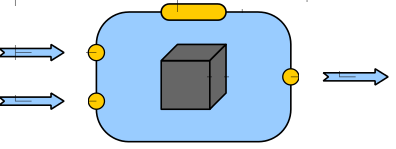
\includegraphics[width=0.5\textwidth]{block.png}
\end{figure}    
\end{columns}
\end{frame}


\begin{frame}
\frametitle{Формальное описание разрабатываемой модели Workflow}

\textbf{Пример схемы workflow для задачи оптимизации}:
\begin{figure}[here]
    \centering
    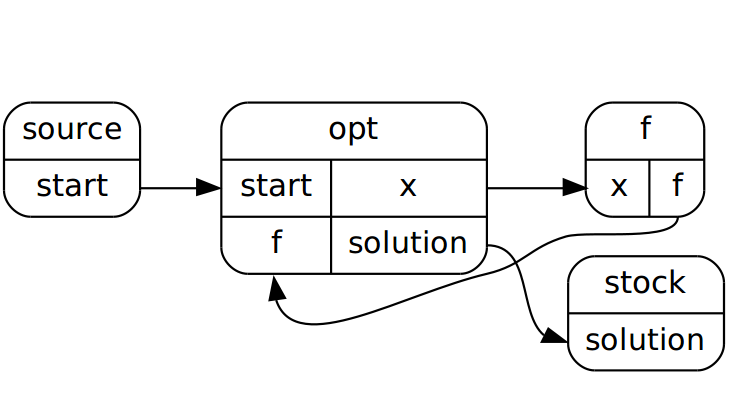
\includegraphics[width=0.5\textwidth]{optimization_workflow.png}
\end{figure}   
\end{frame}


\begin{frame}
\frametitle{Формальное описание разрабатываемой модели Workflow}

\textbf{Конечный автомат блока}:
 $M = (\Sigma, I, O, T, s_{0})$ 
\begin{enumerate}
\item[-] $\Sigma$ -набор конечных состояния,
\item[-] $I$ - непустой набор доступных входных портов блока,
\item[-] $O$ - непустой набор доступных выходных портов блока,
\item[-] $I \bigcap O = \varnothing$ - 
\item[-] $s_{0} \in \Sigma$ - начальное состояние,
\item[-] $T: \Sigma \times (2^{I} \backslash \lbrace \varnothing \rbrace) \rightarrow  2^{\Sigma \times 2^{O}}$ отображение сопоставляющее каждому состоянию и набору входных портов набор состояний с соответствующим набором выходных портов.
\end{enumerate}  
\end{frame}



\begin{frame}
\frametitle{Формальное описание разрабатываемой модели Workflow}

\textbf{Граф состояний и переходов для некоторого оптимизирующего блока}:
\begin{figure}[here]
    \centering
    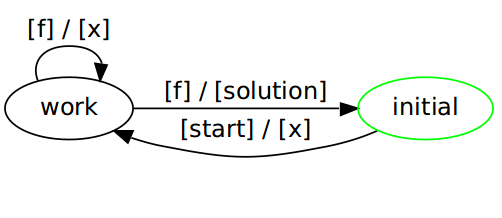
\includegraphics[width=0.5\textwidth]{optimizer_block.png}
\end{figure}  
\end{frame}


\begin{frame}
\frametitle{Формальное описание разрабатываемой модели Workflow}
\textbf{Описание связей в модели}
\begin{itemize}
\item<1-> Cвязи - абстракция передачи данных.
\item<2-> Типы данных на совместимы.
\item<3-> Сигналы по связям передаются мгновенно и без потерь.
\end{itemize} 

\end{frame}

\begin{frame}
\frametitle{Формальное описание разрабатываемой модели Workflow}
\textbf{Некоторые свойства связей}:
\begin{itemize}
\item<1-> Связь может быть установлена только между выходным портом одного блока и входным портом другого блока или самого себя.
\item<2-> Связи могут быть построены как из одного выходного порта ко многим входным, так и из нескольких выходных в один входной порт.
\item<3->Обратим внимание, что если блок испускает сигнал по какому либо порту, то сигнал распространяется по всем связям исходящих, таким образом возможно порождаются конкурирующие потоки.
\item<4-> Входные и выходные порты блоков могут оставаться неподключенными.
\end{itemize} 
\end{frame}

\begin{frame}
\frametitle{Формальное описание разрабатываемой модели Workflow}
\textbf{Граф связей workflow}:
 \begin{itemize}
 \item WFG = $(A, D)$
 \begin{itemize}
 \item A - Набор блоков
 \item D - Набор связей
 \end{itemize} 
 \item<2-> Содержит блоки \textit{Source} и \textit{Stock}.
\end{itemize} 
\end{frame}

\begin{frame}
\frametitle{Формальное описание разрабатываемой модели Workflow}

\textbf{Пример графа связей workflow для задачи оптимизации}:
\begin{figure}[here]
    \centering
    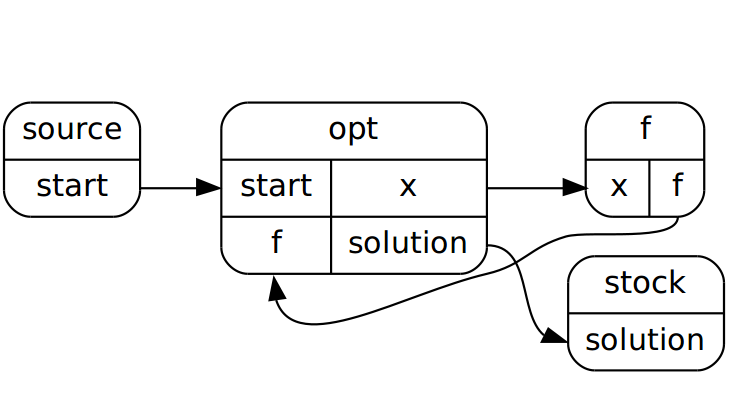
\includegraphics[width=0.5\textwidth]{optimization_workflow.png}
\end{figure}   
\end{frame}

\begin{frame}
\subsection{Возможные ошибки при составлении workflow}
\begin{itemize}
\item<1-3> 
Состояние гонки:
\begin{itemize}
\item<2-3> Случай, когда на один входной порт приходят два сигнала одновременно.
\item<3> Когда на входные порты блока одновременно приходит такой набор сигналов, что что существует неоднозначность запуска.
\end{itemize}

\item<4> Голодание
\begin{itemize}
\item<4> Когда в конце работы workflow остаются необработанные сигналы.
\end{itemize}
\end{itemize}
\end{frame}


\begin{frame}
\frametitle{Анализа разработанной модели workflow}

\begin{figure}[here]
    \centering
    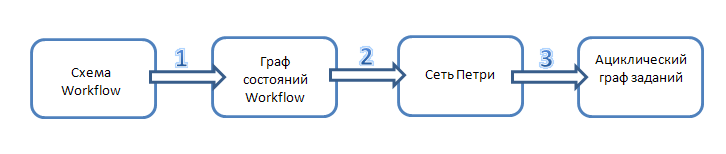
\includegraphics[width=\textwidth]{analys_plan.png}
    \label{img:opt_wf}
\end{figure}

\begin{enumerate}
\item Модифицированный волновой алгоритм
\item Преобразование графа состояний workflow к виду сети Петри
\item Методы избавления от циклов и условных переходов.
\end{enumerate}
\end{frame}

\begin{frame}
\frametitle{Анализа разработанной модели workflow}
\begin{figure}[here]
    \centering
    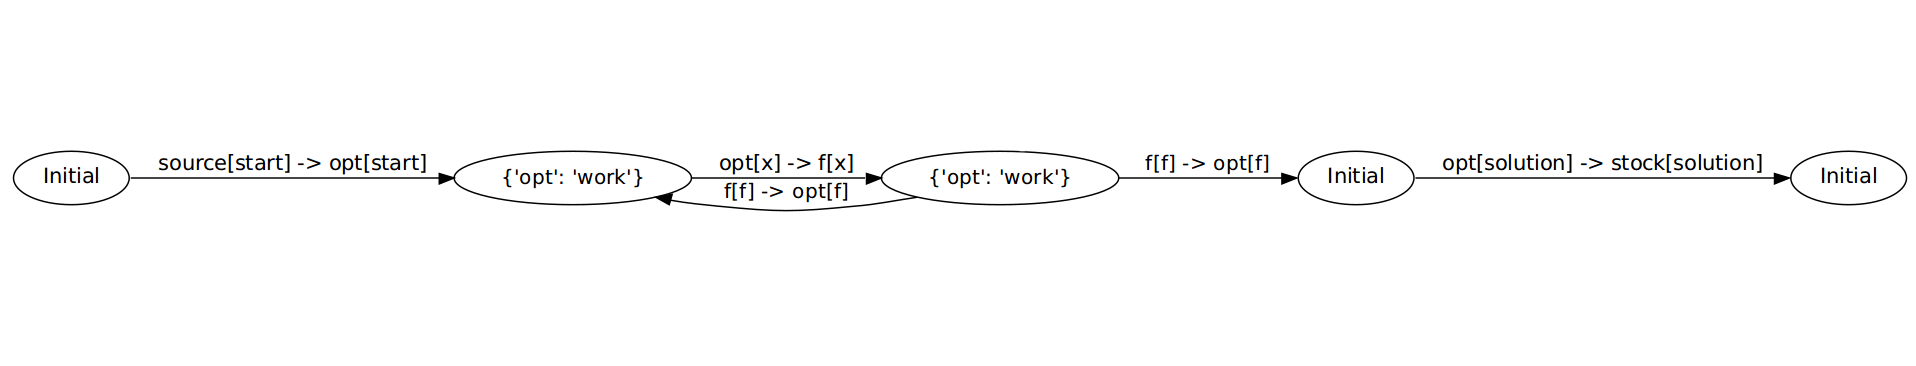
\includegraphics[width=\textwidth]{optimization_state_graph.png} 
    \label{img:opt_wf}
\end{figure}
\end{frame}

\begin{frame}
\frametitle{Анализа разработанной модели workflow}
\end{frame}
\begin{frame}
\frametitle{Анализа разработанной модели workflow}
\textbf{Приведение к сети Петри}:
\begin{figure}[here]
    \centering
    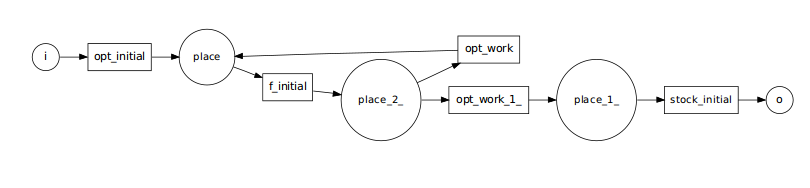
\includegraphics[width=\textwidth]{optimization_petri_net.png} 
    \label{img:opt_wf}
\end{figure}
\end{frame}


\begin{frame}
\frametitle{Анализа разработанной модели workflow}
\textbf{Полученый граф задач}:
\begin{figure}[here]
    \centering
    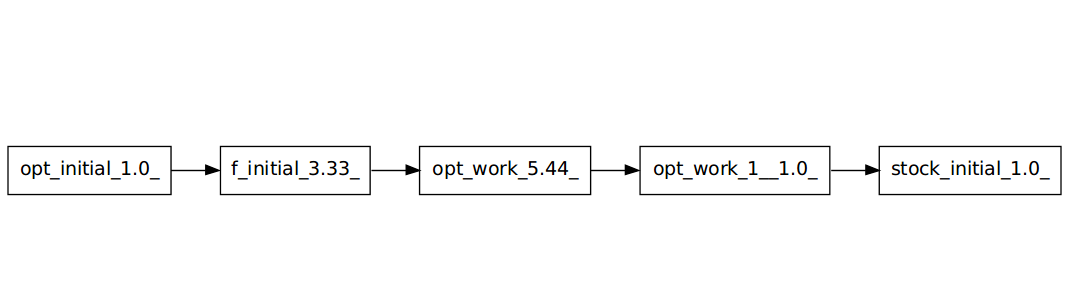
\includegraphics[width=\textwidth]{task_graph.png} 
    \label{img:opt_wf}
\end{figure}
\end{frame}

\begin{frame}
\frametitle{Выработка стратегии запуска}

Стратегия - распределение блоков по узлам.
\begin{enumerate}
\item[•] Считаем , что блоки не переносимы с одного узла на другой.
\item[•] На одном узле может быть запущено несколько блоков, но работать они могут только последовательно.
\item[•] Критерий оценки стратегии - минимальное время работы workflow, c ограничением на утилизацию ресурсов.
\end{enumerate}
\end{frame}

\begin{frame}
\frametitle{Выработка стратегии запуска}

Стратегия - распределение блоков по узлам.
\begin{enumerate}
\item[•] Считаем , что блоки не переносимы с одного узла на другой.
\item[•] На одном узле может быть запущено несколько блоков, но работать они могут только последовательно.
\item[•] Критерий оценки стратегии - минимальное время работы workflow, c ограничением на утилизацию ресурсов.
\end{enumerate}
\end{frame}




\end{document}